
\section{DISC basics}\label{sec:appendix-disc}
\subsection{Notation}

\begin{itemize}[noitemsep]
    \item  $\mathrm{roman}$ -- predicates standing for blockchain verifiable properties 
    \item \textsc{smallcaps}-- field of a composite, tuple member function
    \item $\Pi^p$ -- proof constructor function
    \item $\mathbb{V}^p$ -- validator function
    \item \texttt{TT\_FONT} -- constant parameter (see appendix \ref{sec:constants})
    \item $\mathit{uint}[d]$ -- left closed, right open integer range $\overline{\left[0,2^d\right)}$
\end{itemize}


\subsection{Sequences}
 
\begin{definition}[sequences \statusgreen]
Define $\tau\{n\}$, the non-polymorphic sequences of length $n$ (non-negative) over any type $\tau$ as an indexing function:
%
\begin{eqnarray}
\tau\{n\} &\defeq& \begin{cases}\nil&\text{ if } n=0\\
\overline{0,n-1}\to \tau &\text{ if } n>0
\end{cases}\\
\tau{+}&\defeq&\bigcup_{n\in \mathbb{Z}^{+}} \tau\{n\}\\
\tau{*}&\defeq&\{\nil\}\cup\tau{+}\\
\end{eqnarray}
%
Length function $\mathit{len}$:
\begin{eqnarray}
\mathit{len}(s)&:&\tau\to\mathit{uint64} \\
\mathit{len}(s)&\defeq& \begin{cases}
0 & \text{ if  } s=\nil\\
n & \text{ if  } s\in\tau\{n\}
\end{cases}
\end{eqnarray}
%
The positional index 'at' function:
\begin{eqnarray}
\idx{}&:&\tau*\to\times\mathit{uint64}\to\tau\\
s\idx{}&:&\overline{0,\mathit{len}(s)-1}\to\tau\\
s\idx{i}&\defeq&s'(i)   
\end{eqnarray}
%
Define the \emph{concatenation} operator '$\concat$':
\begin{eqnarray}
(x\concat y)&:& \overline{0, \mathit{len}(x) + \mathit{len}(y)-1}\to\tau\\
(x\concat y)\idx{i} &\defeq& \begin{cases}x\idx{i} & \text{ if  } 0\leq i< \mathit{len}(x)\\
y\idx{i-\mathit{len}(x)}&\text{ otherwise } 
\end{cases}
\end{eqnarray}
%
Define slices (subsequences) with the range operator '$\rangedel$':
\begin{eqnarray}
(s\idx{o\rangedel o+l})&:&\overline{0, l-1}\to\tau\\
(s\idx{o\rangedel o+l})\idx{i}&\defeq&s\idx{o+i} 
\end{eqnarray}
where 
\begin{eqnarray}
o, l \geq 0\land\\
\mathit{len}(x)\geq o+l
\end{eqnarray}
%
Let us also define empty, prefix and suffix slices:
\begin{eqnarray}
s\idx{x\rangedel x} &\defeq& \nil\\
s\idx{\rangedel x} &\defeq& s\idx{0\rangedel x}\\        
s\idx{x\rangedel}  &\defeq& s\idx{x\rangedel \mathit{len}(s)}
\end{eqnarray}
\end{definition}
%
As a special case byte slices are defined as sequences of 8-bit integers.
%
\begin{definition}[segmentation]
\label{def:segmentation}
Define segment as an at most 32 long byte slice, and define  segmentation of a slice of bytes as the partitioning of the slice into consecutive segments. 
%
Define segment count as the number of segments that cover a byte slice:
\begin{eqnarray}
\mathit{SegCnt}&:&\mathit{byte}*\to\mathit{uint64}\\
\mathit{SegCnt}(s)&\defeq&\mathit{int}\left(\frac{\mathit{len}(s)-1}{32}\right)+1 
\end{eqnarray}
%
Now we can define the segment indexing function 
$\idx{\idx{}}$ which maps the byte slice $s$ and an index $i$ to the $i$-the segment in the segmentation of $s$:
\begin{eqnarray}
\idx{\idx{}}& : & \mathit{byte}{*}\to\mathit{uint64}\to\mathit{Segment}\\
s\idx{\idx{}}&:&\overline{0,\mathit{SegCnt}(s)-1}\to\mathit{Segment}\\ 
s\idx{\idx{i}}&\defeq&\begin{cases}s\idx{32\cdot i\rangedel} &\text{ if } i = \mathit{SegCnt}-1\\
s\idx{32\cdot i\rangedel 32\cdot(i+1)} &\text{otherwise}
\end{cases}
\end{eqnarray}
\end{definition}

\subsection{Custom types}


\begin{definition}[Swarm overlay address of node $n$]\label{def:overlay}
%
A Swarm node is associated a Ethereum account that the node operator must possess the private key for, called \emph{bzz account} ($K_n^\mathit{bzz}$). The node's overlay address is derived as the hash of the binary serialisation of the Ethereum address of this account with the Swarm network ID and a minable nonce appended. 
%
\begin{eqnarray}
\mathit{overlay}(n) \defeq \mathit{H}(acc\concat id\concat \nu)      
\end{eqnarray}
where
\begin{eqnarray}
\textsc{eth address } acc&=& \mathit{Account}(K_n)\\
\textsc{network id } id&=& \texttt{BZZ\_NETWORK\_ID}\\
\textsc{overlay nonce } \nu&\in&\mathit{Nonce}
\end{eqnarray}
\end{definition}


\begin{definition}[DISC custom types \statusgreen]
Let us define the  DISC specific custom types used in the formalisation.
\begin{itemize}[noitemsep,leftmargin=0pt]
\item[] $\mathit{Segment}\equiv\mathit{byte}\{32\}\equiv\mathit{uint256}$\\\hspace*{1em}
    32-long slice of raw bytes\\\hspace*{1em}
    in numerical context cast as BigEndian encoded 256-bit unsigned integer 
\item[]  $\mathit{Address} \equiv \mathit{Segment}$\\\hspace*{1em}
    swarm chunk address, swarm peers' overlay address
\item[] $\mathit{Nonce} \equiv \mathit{Segment}$\\\hspace*{1em}
    deterministically random $\mathit{Segment}$
% \item[] $\mathit{Chunk}\equiv\mathit{byte}\{,4096\}$\\\hspace*{1em}
% content addressed chunk data; byte array with maximum length of 4K
% \item[] $\mathit{Chunks}\equiv \mathit{Address}\times\mathit{uint64}\times\mathit{Chunk}$\\\hspace*{1em}    
% content addressed chunk or single owner chunk
\item[]$\mathit{Account}\equiv \mathit{byte}\{20\}$\\\hspace*{1em}
    Ethereum address deriveed from EC keypair $K$\\\hspace*{1em}
    $\mathit{Account}(K)\defeq\mathit{H}(\mathit{PubKey}(K))\idx{12\rangedel32}$
\item[] $\mathit{Nodes} \equiv \mathit{Segment}$\\\hspace*{1em}
    swarm client node (peer)
\item[]$\mathit{Sig} \equiv \mathit{byte}\{65\}$\\\hspace*{1em}
$\langle r,s,v\rangle$ representation of an EC signature (32+32+1
bytes)
\item[] $\mathit{Timestamp}\equiv\mathit{uint64}$\\\hspace*{1em}
    64-bit unsigned integer for unix time, nanosecond resolution\\\hspace*{1em} 
    big endian binary serialisation.
\item[] $\mathit{H}:\mathit{byte}{*}\to             \mathit{Segment}$\\\hspace*{1em}
the 256-bit Keccak SHA3 hash function, the base hash used in swarm.
\end{itemize}
\end{definition}

% \newpage

% \subsection{Nodes and overlay address \statusgreen}



\subsection{XOR distance and proximity order\statusgreen}\label{sec:proximity}

\begin{definition}[XOR distance ($\chi$)]\label{def:xor}
Consider the set of bit sequences with fixed length $d$ as points in a space. 
Define a distance metric $\chi$ such that
the distance between two such sequences is the numerical value of their bitwise XOR ($\xor$) using big endian (= most significant bit first) encoding.
\begin{eqnarray}
\chi&:&\mathit{uint}[d] \times\mathit{uint}[d]\to\mathit{uint}[d]\\
\chi(x, y) &\defeq& \mathit{Uint}^{d}(\mathit{BE}
^{d}(x)  \xor \mathit{BE}
^{d}(x)))
\end{eqnarray}

Given the fixed length $d>0$, there is a maximum distance ($2^d-1 = \chi(0\{d\},1\{d\})$) in this space, and thus we can define the notion of \emph{normalised distance}:
%
\begin{eqnarray}
\overline{\chi}&:& \mathit{uint}[d] \times\mathit{uint}[d]\to\mathbb{Q}[0,1]\\
\overline{\chi}(x, y) &\defeq &\frac{\chi(x,y)}{2^d-1}
\end{eqnarray}
\end{definition}



\begin{definition}[Proximity order ($\mathit{PO}$) \statusgreen]
\label{def:xorPO}
Proximity order (PO) is a discrete logarithmic scaling of proximity.
%
\begin{eqnarray}
\mathit{PO}&:& \mathit{uint}[d] \times\mathit{uint}[d]\to \overline{0,d}\\
\mathit{PO}(x,y) &\defeq &
\begin{cases}
d & \text{ if } x=y\\
\mathit{int}(\log_2(\mathit{Proximity}(x, y)))&\text{otherwise}\\
\end{cases}
\end{eqnarray}
%
where proximity is the inverse of normalised distance:
%
\begin{eqnarray}
\mathit{Proximity}&:& \mathit{uint}[d] \times\mathit{uint}[d]\to \mathit{uint}[d]\\
\mathit{Proximity}(x, y) &\defeq & \frac{1}{\overline{\chi}(x,y)}
\end{eqnarray}

Given two points $x$ and $y$,  the order of their proximity $\mathit{PO}(x,y)$ equals the number of initial bits shared by their respective most significant bit first binary representations. In practice, with $d=256$,  $\mathit{uint}[d]\equiv\mathit{Segment}$, so $\mathit{PO}$ also applies to a pair of  slices of 32 bytes.
\end{definition}


\subsection{Binary Merkle tree hash}

\begin{figure}[!ht]
   \centering
   \resizebox{.85\textwidth}{!}{
   \tikzset{
level/.style={
  sibling distance={(width("$H^126$")+4pt)},
  level distance=15mm,
  line width=.5pt,
},
mtnode/.style={
  minimum width={width("$H^126$")+2pt},
  minimum height={.7cm},
  inner sep=2pt,
  outer sep=2pt,
  rectangle,
  rounded corners=1pt,
  draw,
  line width=.7pt
},
% edge from parent/.style={draw=none},
mtedge/.style={grow=down,draw=none,<-, edge from parent/.style={draw}},
link/.style={draw=none, edge from parent/.style={draw=none}},
mtedgeadj/.style={mtedge, shorten >=10pt  },
mpedge/.style={mtedge, line width=.7pt,densely dashed},
ellip/.style={draw,loosely dotted, shorten >=5mm, thick,<-, edge from parent/.style={draw}},
bubble/.style={minimum height={1cm}, draw=none, align=center},
data/.style={mtnode,fill=gray!50,line width=.7pt},
mppath/.style={mtnode,line width=.7pt},
mpext/.style={mtnode,line width=.7pt},
mpdata/.style={data,line width=.7pt},
mpdataext/.style={data,line width=.7pt}
}

\begin{tikzpicture}
                  % level 7
\node[mtnode](bmtroot){$H_R$}
  child[<-,grow=left,level distance=3cm] { node[bubble] (ash) {BMT Chunk Hash}  }
  child[grow=down]{ node[mtnode] at (-2,0)(root) {$1337$}
    child[<-,grow=left,level distance=3cm] { node[bubble] (ash) {8 byte span}  }
  }
  child[grow=down]{ node[mtnode] at (2,0) (root) {$H^7_0$}
                  % level 6
  child[<-,grow=right,level distance=3cm] { node[bubble] (ash) {BMT Root}  }
  child { node[mppath] (6-0) {$H^6_0$}   % 0
                  % level 5
    child { node[mppath] (5-0) {$H^5_0$}          % 0
      % child[mpedge]
                  % level 4
                  % mppath goes the other way
      child { node[mpext] (4-0) {$H^4_0$}
        % % child[mtedgeadj]
                  % level 3
        child { node[mtnode] (3-0) {$H^3_0$}
              % level 2
          child { node[mtnode] (2-0) {$H^2_0$}
                % level 1
            child { node[mtnode] (1-0) {$H^1_0$}
                % level 0
              child { node[mtnode] (0-0) {$D^0_0$}
                % data level
                child[mtedge] { node[text width=3cm, align=center] (c-0) {32 byte segments.} }
              }
              % % child[mtedgeadj]
              child { node[mtnode] (0-1) {$D^0_1$}
              }
                % level 0
            }
                % level 1
            % child[mtedgeadj]
            child { node[mtnode] {$H^1_{1}$} child[ellip] }
          }
                % level 2
          % child[mtedgeadj]
          child { node[mtnode] {$H^2_{1}$} child[ellip] }
        }
                % level 3
        % child[mtedgeadj]
        child { node[mtnode] {$H^3_{1}$} child[ellip] }
      }
                % level 4
      child[missing]
      child[missing]
      child { node[mppath] (4-1) {$H^4_1$}                 % 1
                % level 3
        child { node[mpext] (3-4) {$H^3_4$} child[ellip] }
        % child[mpedge]
        child { node[mppath] (3-5) {$H^3_5$}  % 1
                % level 2
          % child[mpedge]
          child { node[mppath] (2-10) {$H^2_{10}$}           % 0
                % level 1
            child { node[mpext] (1-21) {$H^1_{21}$} child[ellip] }
            % child[mpedge]
            child { node[mppath] (1-22) {$H^1_{22}$}         % 1
                % level 0
              child { node[mppath] (0-42) {$D^0_{42}$}       % 0
              }
                % level 0
              % child[mpedge]
              child { node[mpext] (0-43) {$D^0_{43}$}
              }
                % level 0
            }
                % level 1
          }
                % level 2
          % child[mpedge]
          child { node[mpext] (2-11) {$H^2_{11}$} child[ellip] }
        }
                % level 3
        % child[missing]
      }
                % level 4
    }
                % level 5
    child[missing]
    % child[mpedge]
    child[missing]
    child { node[mpext] (5-1) {$H^5_1$} child[ellip] }
  }
                % level 6
  child[missing]
  child[missing]
  % child[mtedgeadj]
  child[missing]
  child  { node[mpext] (6-1) {$H^6_1$}
                % level 5
    child { node[mtnode] (5-2) {$H^5_2$} child[ellip] }
    child[missing]
    % child[mtedgeadj]
    child { node[mtnode] (5-3) {$H^5_3$}
                % level 4
      child { node[mtnode] {$H^4_{6}$} child[ellip] }
      % child[mtedgeadj]
      child { node[mtnode] (4-7) {$H^4_7$}
                % level 3
        child { node[mtnode] {$H^3_{14}$} child[ellip] }
        % child[mtedgeadj]
        child { node[mtnode] (3-15) {$H^3_{15}$}
                % level 2
          child { node[mtnode] {$H^3_{30}$} child[ellip] }
          % child[mtedgeadj]
          child { node[mtnode] (2-31) {$H^2_{31}$}
                % level 1
            child { node[mtnode] {$H^1_{62}$} child[ellip] }
            % child[mtedgeadj] {node {}}
            child { node[mtnode] (1-63) {$H^1_{63}$}
                % level 0
              child { node[mtnode] (0-126) {$D^0_{126}$}
              }
              % child[mtedgeadj]
              child { node[mtnode] (0-127) {$D^0_{127}$}
                child { node[draw=none, text width=6cm, align=center] (spanann) {zero padding if needed to fill 4Kb.} }
              }
                % 0
            }
                % 1
          }
                % 2
        }
                % 3
      }
                % 4
    }
               % 5
  }
}               % 6
 ;
\end{tikzpicture}}
   \caption[BMT: Binary Merkle Tree hash]{BMT (Binary Merkle Tree) used as the native chunk hash in Swarm. In this example, 1337 bytes of chunk data is segmented into 32 byte segments. Zero padding is used to fill up the rest up to 4 kilobytes. Pairs of segments are hashed together using the ethereum-native Keccak256 hash to build up the binary tree. On level 8, the binary Merkle root is prepended with the 8 byte span and hashed to yield the BMT chunk hash.}
   \label{fig:BMT}
\end{figure}

The BMT chunk address is the hash of the 8 byte metadata (span) and the root hash of a \emph{binary Merkle tree} (\emph{BMT}) built on the 32-byte segments of the underlying data (see figure \ref{fig:BMT}). If the chunk content is less than 4k, the hash is calculated as if the chunk was padded with all zeros up to 4096 bytes.


\begin{definition}[Binary Merkle Tree Root \statusgreen]
\label{def:bmtroot}
Define  $\triangle[\mathit{H},n](i,d)$ as the Binary Merkle Tree Root of data $d$ fitting in at most $2^n$ 32-byte segments using $\mathit{H}$ as its base hash:
%
\begin{eqnarray}
\triangle&: &(\mathit{byte}{*}\to\mathit{Segment})\times\mathit{uint8}\to\mathit{uint8}\times\mathit{byte}{*} \to \mathit{Segment} 
\\
\triangle[\mathit{H},n]=&:&\overline{0,n}\times\mathit{byte}\{,2^{n}\}\to \mathit{Segment} \\
\triangle[\mathit{H},n](i,d) &\defeq &\begin{cases}d &\text{if }i=0
\\
\triangle[\mathit{H},n](i,d\concat 0\{2^{n+5}-\mathit{len}(d)\})& \text{if }\mathit{len}(d)<2^{i+5} \\
\mathit{H}(\triangle[\mathit{H},n](d\idx{\rangedel 2^{i-1}},i-1)\concat\\
\ \ \concat  \triangle[\mathit{H},n](d\idx{2^{i-1}\rangedel},i-1)) & \text{otherwise }
\end{cases}
\end{eqnarray}
\end{definition}

\begin{definition}[Binary Merkle Tree Hash \statusgreen]
\label{def:bmt}
Define  $\mathit{BMT}[H](d,m)$ as the hash of Binary Merkle Tree Root of chunk length data $d$ prepended with metadata $m$.  $H$ is the base hash function, by default 256-bit Keccak. Note that a chunk size blob of bytes can accommodate 128 32-byte segments, hence  depth $7$:
%
\begin{eqnarray}
\mathit{BMT}&:&(\mathit{byte}{*}\to\mathit{Segment})\to  \mathit{Chunk}\times\mathit{byte}\{8\}\to\mathit{Segment}\\
\mathit{BMT}[\mathit{H}] &:&\mathit{Chunk}\times\mathit{byte}\{8\}\to\mathit{Segment}\\
\mathit{BMT}[H](d,m)&\defeq&\mathit{H}(m\concat \triangle[\mathit{H},7](7,d))
\end{eqnarray}

\end{definition}

\subsection{Chunks}

\begin{definition}[Content addressed chunks \statusgreen]
\label{def:cac}
Define content address chunk $c$ as a function from bytes data with size limit of 4096 bytes and an associated address calculated with BMT:
% 
\begin{eqnarray}
\mathit{CAC} &:& \mathit{Chunk}\times\mathit{byte}\{8\}\to\mathit{Chunks}\\
\mathit{CAC}(d,m)&\defeq&\langle addr,cont\rangle
\end{eqnarray}
%
such that
%
\begin{eqnarray}
addr&\defeq&\mathit{BMT}(d,m)\\
cont&\defeq&m\concat d
\end{eqnarray}


By convention the metadata prefix $m$ encodes the \emph{span} using 64-bit little endian. If the chunk is an intermediate chunk (see definition \ref{def:pac}), the span is the length of the data that the subtree spans over. If the chunk is a data chunk, then span encodes the data length:
%
\begin{eqnarray}
m&\defeq& \mathit{LE}^{64}(\mathit{len}(d))
\end{eqnarray}

We also say that for $cac = \mathit{CAC}(d,m) = \langle addr,cont\rangle$:
%
\begin{eqnarray}
\textsc{address}(cac)&\defeq&addr\\
\textsc{payload}(cac)&\defeq&cont\\
\textsc{data}(cac)&\defeq& d\\
\textsc{metadata}(cac)&\defeq& m
\end{eqnarray}

For convenience \emph{SegCnt} and the segment indexing function '\idx{\idx{}}' can be trivially extended to apply to chunks:
%
\begin{eqnarray}
\mathit{SegCnt}&:&\mathit{Chunks}\to\mathit{uint64}\\
\mathit{SegCnt}(c)&\defeq&\mathit{SegCnt}(\textsc{data}(c))
\end{eqnarray}

\begin{eqnarray}
\idx{\idx{}}&:&\mathit{Chunks}\times\mathit{uint64}\to\mathit{Segment}\\
c\idx{\idx{i}}&\defeq&\textsc{data}(c)\idx{\idx{i}}
\end{eqnarray}
\end{definition}

\subsection{Single Owner Chunks}

\begin{definition}[Single owner chunks \statusgreen]
\label{def:soc}
A single owner chunk  is defined as a content addressed chunk associated with an ID and an ethereum address: 
%
\begin{eqnarray}
\mathit{SOC} &\defeq& \mathit{Account}\times\mathit{Segment}\times\mathit{CAC}\to\mathit{Chunks}\\
\mathit{SOC}(owner,id,cac)&\defeq& \langle addr, cont\rangle
\end{eqnarray}
%
where
%
\begin{eqnarray}
addr&\defeq& \mathit{H}(o\concat id)\\
cont &\defeq& id\concat\mathit{Sig}(o, id\concat\textsc{address}(cac))\concat \textsc{payload}(cac)
\end{eqnarray}

A single owner chunk's address is the Keccak256 hash of identifier prepended to owner account, while its data is serialised as follows:
\begin{itemize}[noitemsep]
    \item[--] \emph{identifier} -- 32 bytes arbitrary identifier, 
    \item[--] \emph{signature} -- 65 bytes $\langle r,s,v \rangle$ representation of an EC signature (32+32+1 bytes),
    \item[--] \emph{span} -- 8 byte little endian binary of uint64 chunk span,
    \item[--] \emph{data} -- max 4096 bytes of regular chunk data.
\end{itemize}

Integrity of a \emph{single owner chunk} is verified with the following process:
\begin{enumerate}[noitemsep]
    \item Deserialise the chunk content into fields for identifier, signature and payload.
    \item Construct the expected plaintext composed of the identifier and the \emph{BMT hash} of the payload.
    \item Recover the owner's address from the signature using the plaintext.
    \item Check the hash of the identifier and the owner (expected address) against the chunk address.
\end{enumerate}

\end{definition}

\begin{definition}[Packed address chunk\statusgreen]
\label{def:pac}
Define the packed address chunk for a sequence of chunks $C$ as the concatenation of all the addresses of the chunks in the sequence:
%r
\begin{eqnarray}
\mathit{PAC}&:&\mathit{Chunks}{*}\times\mathit{byte}\{8\}\to\mathit{Chunks}\\
\mathit{PAC}(C,m)&\defeq&\mathit{CAC}\left(\Concat_{i=0}^{\mathit{len}(C)-1} \mathit{Address}(C\idx{i}), m\right)
\end{eqnarray}
\end{definition}

\subsection{Segment inclusion proofs}

Using BMT hashes allows for compact \emph{segment inclusion proofs} (substring relationship with a 32-byte resolution).

\begin{figure}[!ht]
\centering
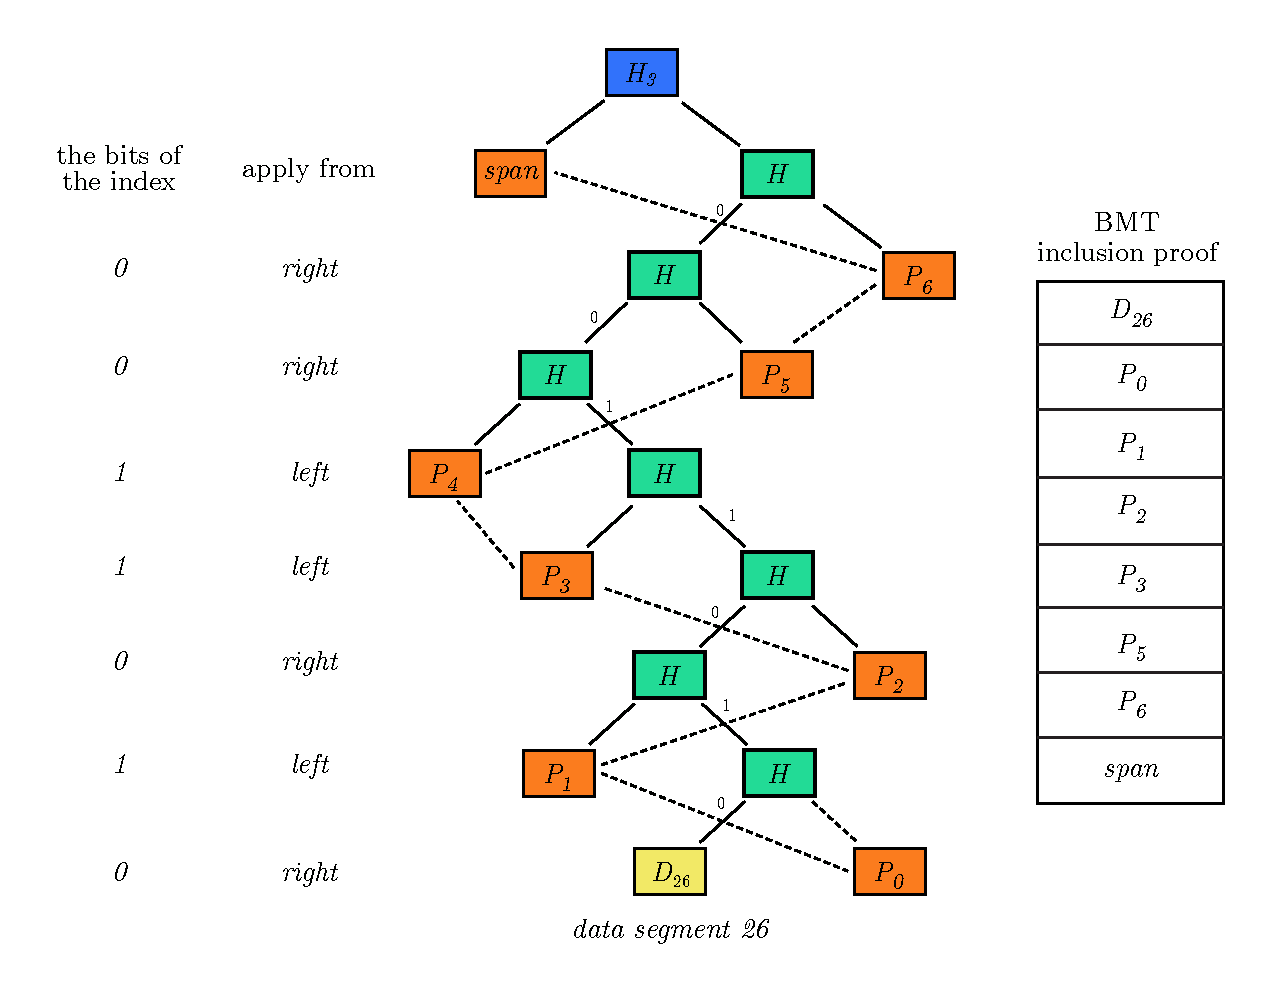
\includegraphics[width=.85\textwidth]{fig/inclusion-proof.pdf}
\caption[Compact segment inclusion proofs for chunks ]{Compact segment inclusion proofs for chunks. Assume we need proof for segment 26 of a chunk (yellow). The orange hashes of the BMT are the sister nodes on the path from the data segment up to the root and constitute what needs to be part of a proof. When these are provided together with the root hash and the segment index, the proof can be verified. The side on which proof item $i$ needs to be applied depends on the $i$-th bit (starting from least significant) of the binary representation of the index. Finally the span is prepended and the resulting hash should match the chunk root hash.}
\label{fig:chunk-inclusion}
\end{figure}

\begin{definition}[BMT segment inclusion proof \statusgreen]
\label{def:sip}
Define  $\proofof{sip}(c,i)$ as the $\mathit{BMT}$ inclusion proof on chunk $c$ for segment index $i$:
%
\begin{eqnarray}
\proofof{sip}&: &\mathit{Chunks}\times \overline{0,127} \to \mathit{SIP}\\
\mathit{SIP}&\defeq&\mathit{Segment}\times\mathit{Segment}^7\times \mathit{byte}\{8\}
\\
\proofof{sip}(c,i) &\defeq &\langle c\idx{\idx{i}},\langle h_0, h_1, \ldots, h_6\rangle, \textsc{metadata}(c)\rangle  
\end{eqnarray}
%
where
%
\begin{eqnarray}
h_j&\defeq& \mathit{BMT}(s_j,j)\\
s_j&\defeq&c\idx{\mathit{start}(i,j)\rangedel\mathit{start}(i,j)+32\cdot 2^j}
\end{eqnarray}
%
where
%
\begin{eqnarray}
\mathit{start}(i,j)&\defeq&
\begin{cases}
0 &\text{if } j=7\\
start(i,j+1) & \text{if } \mathit{int}\left(i / 2^j\right) = 0 \mod 2\\
start(i,j+1)+32\cdot 2^{j} &\text{otherwise}
\end{cases}
\end{eqnarray}
\end{definition}

In order to validate segment inclusion proofs we first introduce the prover hash function $\mathit{H}_{\Pi}$.

\begin{definition}[BMT prover function\statusgreen]
\label{def:prover-function}
%
\begin{eqnarray}
\mathit{H}_{\Pi}&:&\overline{0,127}\times\mathit{SIP}\to\mathit{Address}\\
\mathit{H}_{\Pi}(i,\langle d, sisters, m\rangle)&\defeq&\mathit{H}(m,\mathit{H}_{\Pi}^{\triangle}(7,d,sisters))
\end{eqnarray}
%
where
%
\begin{eqnarray}
\mathit{H}_{\Pi}^{\triangle}&:&\overline{0,7}\times\mathit{Segment}\times\mathit{Segment}^7\to\mathit{Address}\\
\mathit{H}_{\Pi}^{\triangle}(j,d,s)&\defeq& \begin{cases}
d & \text{ if } j=0\\
\mathit{H}(\mathit{H}_{\Pi}^{\triangle}(j-1,d,s)\concat s\idx{j-1}) & \text{if }\mathit{int}(i/2^{j-1}) = 0 \mod 2\\
\mathit{H}(s\idx{j-1}\concat \mathit{H}_{\Pi}^{\triangle}(j-1,d,s)) &\text{otherwise}
\end{cases}
\end{eqnarray}
\end{definition}


\begin{definition}[BMT SIP validation \statusgreen]
\label{def:sip-validation}
Define  $\validator{sip}(a, i, p)$ as the validator of a BMT segment inclusion proof $p$ for chunk at address $a$ on segment index $i$:
%
\begin{eqnarray}
\validator{sip}&:&\mathit{Segment}\times\overline{0,127}\times \mathit{SIP} \to \{\mathtt{T,F}\}
\\
\validator{sip}(a,i,p) &\Leftrightarrow&
\mathit{H}_{\Pi}(i,p)=a
\end{eqnarray}
\end{definition}

\begin{definition}[Single owner chunks data integrity proof \statusgreen]
\label{def:socproof}
Define a single owner chunk storage proof $\proofof{soc}(c,i)$ as a segment inclusion proof of the data payload of SOC $c$ on index $i$ together with the ID and signature of SOC $c$:
%
\begin{eqnarray}
\mathit{SIP}_\mathit{SOC} &\defeq&\mathit{SIP}\times\mathit{Sig}\times\mathit{Segment}\\
\proofof{sip[soc]} &:&\mathit{SOC}\times\overline{0,127}\to\mathit{SIP}_\mathit{SOC}\\ 
\proofof{sip[soc]}(\langle o,id,cac\rangle,i)&\defeq&  \langle p, sig, id\rangle
\end{eqnarray}
%
where
%
\begin{eqnarray}
p&=&\proofof{sip}(cac,i)\\
sig&=&\mathit{Sig}(o,id\concat \mathit{address}(cac))
\end{eqnarray}
\end{definition}

\begin{definition}[Single owner chunks data integrity validation  \statusgreen]
\label{def:socproof-validity}
Define $\validator{sip[soc]}(a, i, p)$ as the validator of a single owner chunk storage proof $p$ for chunk at address $a$ on segment index $i$:
%
\begin{eqnarray}
\validator{sip[soc]}&:&\mathit{Address}\times\overline{0,127}\times\mathit{SIP}_\mathit{SOC}\to\{\texttt{T,F}\}\\ \validator{sip[soc]}(a, i, \langle p, sig, id\rangle)&
\Leftrightarrow&a= \mathit{H}(id\concat o)
\end{eqnarray}
such that 
\begin{eqnarray}
\textsc{owner } o&=& \mathit{ECRecover}(sig,id\concat a')\\
\textsc{payload } a'&=& \mathit{H}_{\Pi}(i,p)
% \\
% \textsc{proof } p&=&\langle d, sisters, m\rangle
\end{eqnarray}
\end{definition}



\subsection{Postage stamps}
\begin{definition}[Postage stamps \statusgreen]
\label{def:postage-stamp}
%
\begin{eqnarray}
\mathit{Stamps}&\defeq& \mathit{Segment}\times\mathit{uint64}\times\mathit{Timestamp}\times\mathit{Address}\\
\mathit{ps} &=&\langle  b,i,ts,a\rangle\in \mathit{Stamps} 
\\
\textsc{batchID}(ps) &\defeq& b 
\\
\textsc{index}(ps) &\defeq &i 
\\
\textsc{timestamp}(ps)&\defeq &ts 
\\
\textsc{address}(ps) &\defeq &a 
\end{eqnarray}
\end{definition}


\begin{definition}[Storage slot reference \statusgreen]
\label{def:slot}
Define the \emph{storage slot reference} $\mathit{slot}(ps)$ of a postage stamp $ps$ as the tuple of the batch identifier and the within-batch stamp counter:
%
\begin{eqnarray}
\mathit{Slots}&\defeq&\mathit{Segment}\times\mathit{uint64}\\
\mathit{slot}&:& \mathit{Stamps}\to\mathit{Slots}\\
\mathit{slot}(ps) &\defeq &\langle \textsc{batchID}(ps),\textsc{index}(ps)\rangle 
\end{eqnarray}
%
% Naturally storage slot reference of a chunk $\mathit{slot}(c)$ is defined as the slot reference of the postage stamp attached to the chunk.
\end{definition}


\begin{definition}[Postage stamp validity \statusgreen]
\label{def:postage-stamp-validity}
Define $\validator{stamp}(ps)$ as the validator of the proof of relevance expressed as the postage stamp $ps$ relying on blockchain information:
%
\begin{eqnarray}
\validator{stamp}&:& \mathit{Stamps} \times\Gamma\times\mathit{Nodes}\to \{\mathtt{T,F}\}\\
\validator{stamp}(ps,\gamma,n) &\Leftrightarrow& \\
\textsc{authentic} & & \textsc{batchID}(ps)\in\mathrm{Batches}(\gamma)\wedge
\\
\textsc{alive} & & \mathrm{Balance}(ps) > 0 \wedge 
\\
\textsc{authorised} & &  \mathit{ECRecover}(\mathit{Sig}(ps), \mathit{encode}(ps)) = \mathrm{Owner}(ps) \wedge
\\
\textsc{available} & & 0 <= \textsc{index}(ps) < \mathrm{Size}(ps)\wedge
\\
\textsc{aligned} & & \mathit{PO}(\textsc{index}(ps),n) \geq \textsc{depth}(\mathit{reveal}(\gamma, n))
\end{eqnarray}
\end{definition}

\subsection{Ordering and sampling}


\begin{lemma}[Ordering and indexing functions\statusgreen]
\label{lem:ordering}
Given an arbitrary finite set $C$, and another set $I$ with a total order $<$.
Any invertible function total over $C$, $f: C\to I$ defines a total order $<_f$ over $C$ as follows:
%
\begin{eqnarray}
<_f&\subseteq&C\times C\\
\forall c,c'\in C, c<_f c'&\Leftrightarrow& f(c)<f(c')
\end{eqnarray}

\begin{proof}
$f$ is injective wrt $I$, so $\mathit{Image}(f)=J\subseteq I$. Since $<$ restricted to a subset ($<_J$) is also a total order over $J$.
Since $f$ is invertible, $C$ and $J$ are isomorphic and therefore the total order $<$ on $J$ carries over to $C$. \qedsymbol
\end{proof}
\end{lemma}

\begin{corollary}[hash orders\statusgreen]
Any hash function defines a total order on a finite set of byte slices.
%
\begin{proof}
The collision free nature of the hash function makes it practically invertible. The actual hashes when read as binary encodings of integers, offer a natural integer ordering over the values. 
\end{proof}

Example: the prefixed BMT hash transform (see \ref{def:prefixed-hash}) defines a total order over a set of chunks.
\end{corollary}

\begin{definition}[Sampler function]
\label{def:sampler}
%
Using $f$ and its derivative ordering on $C\subseteq\mathit{Dom}(f)$ we represent $C$ as an ordered sequence:
%
\begin{eqnarray}
\overrightarrow{\mathit{Seq}}
&:&(T\to  T)\times\mathcal{P}(T)\to T{*}\\
\overrightarrow{\mathit{Seq}}(f,C) 
&\defeq& C'\\
\text{such that }
f(C'\idx{i})<f(C'\idx{j}) &&\text{ for every } 0\leq i<j<\lvert C\rvert
\end{eqnarray}


Finally, we define a sampler function for any $f$ invertible with an image having a total order and $C\subseteq\mathit{Dom}(f)$ such that it selects a prefix slice of length $l$ from the ordered $C$:         

\begin{eqnarray}
\mathit{Sampler} &:&(T\to  T)\times\mathcal{P}(T)\times \mathit{uint64}\to T{+}\\
% \mathit{Sampler}(f,C) &:&\overline{0,\lvert C\rvert-1}\to T\{,\lvert C\rvert\}\\
\mathit{Sampler}(f,C,l) &\defeq& \overrightarrow{\mathit{Seq}}(f,C)\idx{\rangedel l}
\end{eqnarray}
\end{definition}

\section{Redistribution game}\label{sec:appendix-game}
\label{sec:redistribution-game}

\begin{definition}[Redistribution game round\statusgreen]

\label{def:redistribution-game-round} 
Define $\gamma$ as a redistribution game round.  $\gamma$ is conceived of as a multidimensional index:
%
\begin{eqnarray}
\Gamma&\defeq&\mathit{uint64}\times\mathit{uint64}\times\mathit{uint64}\\
\gamma\in\Gamma&=&\langle c,\sigma,i\rangle\\
\textsc{chain}(\gamma)&c&\text{ID of the blockchain context}\\
\textsc{series}(\gamma)&\sigma&\text{index of the parallel series}\\
\textsc{round}(\gamma)&i&\text{sequential index of the round}
\end{eqnarray}

Define $\textsc{block}(\gamma)$ as the starting block height of this particular game $\gamma$:
%
\begin{eqnarray}
\textsc{block}(\gamma)&\defeq&\textsc{round}(\gamma)\cdot \mathtt{ROUND\_LENGTH}+\mathtt{START\_BLOCK}
\end{eqnarray}

Ordering by sequential index defines the chain of games, which lets us define the $\mathit{Prev}$ function:
%
\begin{eqnarray}
\mathit{Prev}&:&\Gamma\to\Gamma\\
\mathit{Prev}(\langle c,\sigma,i\rangle)&\defeq&\langle c,\sigma,i-1\rangle
\end{eqnarray}
\end{definition}

\subsection{Transactions and on-chain registers}

The smart contract receives transactions from applicants in phases. The following virtual registers capture the information given in these transactions that are relevant for defining the winner:
\begin{itemize}[noitemsep]
\item[--] batches (see definition \ref{def:postage-stamp-validity})
\item[--] stakes (see definition \ref{def:stakes})
\item[--] commits (see definition \ref{def:commits})
\item[--] reveals (see definition \ref{def:reveals})
\end{itemize}

\begin{definition}[Stakes \statusgreen]
\label{def:stakes}
We define $\mathit{Stakes}$ as the registry of stakes resulting from transactions sent to the staking contract. A record is a tuple of a node overlay, the stake balance and the committed stake and can be updated.  
%
\begin{eqnarray}
\mathit{Stakes}&:&\Gamma\to\mathit{Nodes}\times\mathit{uint64}\times\mathit{uint64}\\
\langle n, s, m\rangle\in\mathit{Stakes}(\gamma)&\Leftrightarrow& \\
\textsc{right age}&&\exists b'<b-\mathtt{MIN\_STAKE\_AGE}, \tau\in\mathrm{Transactions}(b') \\
\textsc{node overlay}&& n = \mathit{H}(\mathrm{origin}(\tau)\concat\mathtt{BZZ\_NETWORK\_ID}\concat\mathrm{data}(\tau)\idx{0})\\
\textsc{stake balance}&& s=\mathrm{amount}(\tau)\\
\textsc{committed stake}&& m=\mathrm{data}(\tau)\idx{1}
\end{eqnarray}
%
There is only one stake allowed per node, so we can define the staked amount belonging to a node as the minumum of the stake balance and the committed stake times the unit price of storage:
% 
\begin{eqnarray}
\mathit{Stake}&:&\Gamma\times\mathit{Nodes}\to\mathit{uint64}\\
\mathit{Stake}(\gamma,n)&\defeq&\mathit{min}(s,m\cdot \mathit{Price}(\gamma))
\end{eqnarray}
%
\end{definition}

\begin{definition}[Commits \statusgreen]
\label{def:commits}
We define $\mathit{Commits}(\gamma)$ as the registry of applications for a game $\gamma$ resulting from a transaction sent to the game contract's \emph{commit} endpoint. A tuple of the overlay of the committing node, its commitment hash and the number of the block containing the transaction is entered in the register after verifying that (i) the transaction was sent during the commit phase (right time), and (ii) that the node has enough stake and is not frozen (right amount).                    
%
\begin{eqnarray}
\mathit{Commits}&:&\Gamma\to\mathit{Nodes}\times\mathit{Segment}\times\mathit{Blocks}\\
\langle n,h,b\rangle\in\mathit{Commits}(\gamma)&\Leftrightarrow&%\text{$n$ submitted $h$ as their commit}
\\
% &&\text{during the commit phase}\\
\textsc{right time}
&&b < \mathtt{PHASE\_LENGTH} \mod \mathtt{ROUND\_LENGTH} \\
\textsc{right amount}&&\mathit{stake}(\gamma,n)\geq \texttt{MINIMUM\_STAKE}\\
(\textsc{redundancy})&&
\end{eqnarray}
\end{definition}

\begin{definition}[Reveals\statusgreen]
\label{def:reveals}
We define $\mathit{Reveals}$ as the registry of reveals resulting from a transaction sent to the game contract's reveal endpoint. The reveal record is a tuple of the node overlay, the two commitment hashes, the self-reported storage depth, a serial index used for sorting, the obfuscation key, and the block number. The record is entered in the register after it is validated that (i) it was submitted during the reveal phase (right time), (ii) the commitments when obfuscated match the commit by the same node (right reveal), and (iii) that the neighbourhood selection anchor falls within the node's area of responsibility using the self-reported depth (right location). 
%
\begin{eqnarray}
\mathit{RevealEntry}&:&\mathit{Nodes}\times\mathit{Address}^2\times\mathit{uint8}^2\times\mathit{Nonce}\times\mathit{Blocks}\\
\mathit{Reveals}&:&\Gamma\to\mathcal{P}(\mathit{RevealEntry})\\
r=\langle n,chc,chs,sd,i,k,b\rangle\in\mathit{Reveals}(\gamma)&\Leftrightarrow& 
% \text{ $n$ reveals $chc, chs, sd$  as their commitment}\\
\langle\\
\textsc{node}(r)&=&n\\
\textsc{chc}(r)&=&chc\\
\textsc{chs}(r)&=&chs\\
\textsc{depth}(r)&=&sd\\
\textsc{index}(r)&=&i\\
\textsc{nonce}(r)&=&k\\
\textsc{block}(r)&=&b\\
&&\rangle\\
&\Leftrightarrow&\\
\textsc{right time}
&&p \leq b < 2p \mod r\\
&& p = \mathtt{PHASE\_LENGTH}, r= \mathtt{ROUND\_LENGTH} \\
\textsc{right reveal}&&\mathit{H}(n\concat sd\concat chc\concat chs\concat k)=h \text{ such that }\\
&&\langle n,h,b'\rangle\in\mathit{Commits}(\gamma)\text{ for some }b'\\
\textsc{right location}&&\mathit{PO}(\mathit{addr}(n),\mathit{NSA}(\mathit{Prev}(\gamma)))\geq sd\\
(\textsc{responsibility})&&
\end{eqnarray}
%
There is only one reveal allowed per node, so we can define the reveal belonging to a node:
%
\begin{eqnarray}
\mathit{Reveal}&:&\Gamma\times\mathit{Nodes}\to\mathit{RevealEntry}\\
\mathit{Reveal}(\gamma, n)&=&r
\end{eqnarray}
such that 
\begin{eqnarray}
n&=&\mathit{Node}(r)\\
r&\in&\mathit{Reveals}(\gamma)
\end{eqnarray}
\end{definition}

\subsection{Random nonces}

\begin{definition}[Random nonces for the round\statusgreen]
\label{def:nonce-round}

From the round's random seed (see definition \ref{def:random-seed} appendix \ref{sec:randomness}) we can derive all the necessary random input nonces:
%
\begin{eqnarray}
\textsc{ N.hood Selection Anchor   }\mathit{NSA}(\gamma)&\defeq&\mathit{H}(\mathcal{R}(\gamma)\concat BE^{64}(\mathit{SK}(\gamma)))\\
\textsc{ Truth Selection Nonces  }\mathit{TSN}(\gamma)&\defeq&\mathit{H}(\mathcal{R}(\gamma)\concat\mathit{BE}^{8}(0)) \\
\textsc{ Winner Selection Nonces  }\mathit{WSN}(\gamma, i)&\defeq&\mathit{H}(\mathcal{R}(\gamma)\concat\mathit{BE}^{8}(1)) \\
\textsc{ Reserve sampling salt } \mathit{RSS}(\gamma)&\defeq&\mathit{H}(\mathcal{R}(\gamma)) \\
\textsc{ Segment Selection Nonce } \mathit{SSN}(\gamma,i)&\defeq&\mathit{H}(\mathcal{R}(\gamma)\concat\mathit{BE}^{8}(i))
\end{eqnarray}
where 
\begin{eqnarray}
\mathit{SK}&:&\Gamma\to\mathit{uint64}\\
\mathit{SK}(\gamma)&\defeq&\begin{cases}0&\text{if }\lvert\mathit{Reveals}(\gamma)\rvert>0\\
\mathit{SK}(\mathit{Prev}(\gamma))+1&\text{otherwise}
\end{cases}
\end{eqnarray}

Let us now define the witness selection function $\mathcal{W}$ that selects two random witness indexes as well as the last index of the reserve sample such that they are all distinct:
%
\begin{eqnarray}
\mathcal{W}&:&\Gamma\times\mathit{uint64}\times\{0,1,2\}\to\mathit{uint8}\\
\mathcal{W}(\gamma,m,k)&\defeq&\begin{cases}
\mathit{SSN}(\gamma,0) \mod m-1&\text{ if }k=0\\
m-1&\text{ if }k=2\\
m-2&\text{ if }k=1 \land\\
& \mathit{SSN}(\gamma,0)=\mathit{SSN}(\gamma,1) \mod m-1\\
\mathit{SSN}(\gamma,1) \mod m-2&\text{ otherwise }
\end{cases}
\end{eqnarray}
\end{definition}

% \subsection{Reserve Size}

% \begin{definition}[Network reserve size]
% \label{def:reserve-size}
% Define $\mathrm{ReserveSize}(\gamma)$, the network reserved capacity as the total number of storage slots by all batches valid at block $\mathit{Block}(\gamma)$. This can be read from the batch registry contract:
% %
% \begin{eqnarray}
% \mathrm{ReserveSize}&:&\Gamma\to \mathit{uint64}\\
% \mathrm{ReserveSize}(\gamma)&\defeq&\Sigma_{b\in \mathit{Batches}(\gamma)}\mathrm{Size}(b,\gamma)
% \end{eqnarray}
% \end{definition}


% \begin{definition}[Reserve depth]
% \label{def:reserve-depth}
% Define $\mathrm{ReserveDepth}(\gamma)$ as the base 2 log of the number of neighbourhoods needed to provide redundant storage for the volume of chunks corresponding to the network reserve size at block $\mathit{Block}(\gamma)$ given a fixed node storage capacity of depth \texttt{NODE\_RESERVE\_DEPTH}:
% %
% \begin{eqnarray}
% \mathrm{ReserveDepth}&:&\Gamma\to \mathit{uint8}\\
% \mathrm{ReserveDepth}(\gamma)&\defeq&\mathit{int}(\mathit{log}_2(\mathrm{ReserveSize}(\gamma)))-\texttt{NODE\_RESERVE\_DEPTH}
% \end{eqnarray}
% \end{definition}


\subsection{Winner selection and claim validation}

\begin{definition}[Prefixed hash \statusgreen]
\label{def:prefixed-hash}
Define the hash prefixing function $\mathit{prefix}(H,p)$ as a function which when applied to a hash function $\mathit{H}$ and a constant byte slice $p$  outputs a hash function which for every input returns the hash of the input prefixed by $p$ using $H$.
%
\begin{eqnarray}
\mathit{prefix}&: &(\mathit{byte}{*}\to\mathit{Segment})\times\mathit{byte}{*}\to (\mathit{byte}{*}\to\mathit{Segment})
\\
\mathit{prefix}(H,p) &: &\mathit{byte}{*}\to\mathit{Segment}\\
\mathit{prefix}(H,p)(b) &\defeq & H(p\concat b)
\end{eqnarray}

Exceptionally, we define the prefixed version of BMT hash (denoted as $\mathit{BMT}[]$) as one   that uses the prefixed verson of its base hash:
%   
\begin{eqnarray}
\mathit{BMT}[]&: &\mathit{byte}{*}\to\mathit{Chunk}\times\mathit{byte}\{8\}\to\mathit{Segment}\\
\mathit{BMT}[p]&\defeq&\mathit{BMT}[\mathit{prefix}(\mathit{H},p)]
\end{eqnarray}

\end{definition}
    
\begin{definition}[Transformed chunk reserve sample\statusgreen]
\label{def:transformed-reserve}
%
Let us now define the chunk transformation function $\Delta^C(p)$
for a random nonce prefix $p$ as follows: 
%
\begin{eqnarray}
\Delta^C&:&\mathit{Nonce}\to\mathit{Chunks}\to\mathit{Segment}\\
\Delta^C(p)&:&\mathit{Chunks}\to\mathit{Segment}\\
\Delta^C(p)(c)&\defeq&\mathit{BMT}[p](\textsc{data}(c),\textsc{metadata}(c))
\end{eqnarray}
%
Define the transformed reserve sample $\mathit{RS^C}(\gamma,n)$ for game $\gamma$ and node $n$ as the first  $2^d$ chunks of the node's reserve at block $\textsc{block}(\gamma)$, using the ordering defined (see lemma \ref{lem:ordering} and definition \ref{def:sampler}) by the hash (see definition \ref{def:prefixed-hash}) of their data  using BMT with 256-bit Keccak prefixed with random nonce $p$ as its base hash.
%
\begin{eqnarray}
\mathit{RS^C}&:&\Gamma\times\mathit{Nodes}\to\mathit{Chunks}{*}\\\
\mathit{RS^C}(\gamma,n)&\defeq&\mathit{Sampler}(\Delta^C(p),\mathit{Reserve}(\gamma,n),2^d)
\end{eqnarray}
where 
\begin{eqnarray}
d & = & \texttt{SAMPLE\_DEPTH} \text{ (see \ref{sec:constants})} \\
p & = & \mathit{RSS}(\gamma) \text{ (see definition \ref{def:nonce-round})}
\end{eqnarray}
\end{definition}


\begin{definition}[Chunk reserve sample commitment hash \statusgreen]
\label{def:chc}
Define $\mathit{CH^C}(\gamma,n,)$ for game $\gamma$ and node $n$ as the BMT chunk hash of the packed address chunk (see definition \ref{def:pac}) packing the chunks of the transformed reserve sample (see definition \ref{def:transformed-reserve}) for game $\gamma$ and node $n$.
%
\begin{eqnarray}
\mathit{CH^C}&:&\Gamma\times\mathit{Nodes}\to\mathit{Address}\\
\mathit{CH^C}(\gamma,n)&\defeq&\mathit{Address}(\mathit{PAC^C}(\mathit{RS^C}(\gamma, n), p))
    \end{eqnarray}
where
\begin{eqnarray}
p & = & \mathit{RSS}(\gamma) \text{ (see definition \ref{def:nonce-round})}
\end{eqnarray}
and where 
\begin{eqnarray}
\mathit{PAC^C}&:&\mathit{Chunks}{*}\times\mathit{Nonce}\to\mathit{Chunks}\\
\mathit{PAC^C}(C,p)&\defeq&\mathit{CAC}{}\left(\Concat_{i=0}^{\mathit{len}(C)-1} \mathit{Seg}(C\idx{i},p), m\right)
\end{eqnarray}
where
\begin{eqnarray}
\mathit{Seg}(C\idx{i},p) &=& \mathit{Address}(C\idx{i})\concat \Delta^C(p)(C\idx{i}) \\
m & = & \mathit{LE}^{64}(2\cdot32\cdot\mathit{len}(C))
\end{eqnarray}
\end{definition}

\begin{definition}[Transformed slots reserve sample\statusgreen]
\label{def:transformed-slots}
%
Let us now define the slots transformation function $\Delta^S(p)$
for a random nonce $p$ as follows: 
%
\begin{eqnarray}
\Delta^S&:&\mathit{Nonce}\to\mathit{Chunks}\to\mathit{Segment}\\
\Delta^S(p)&:&\mathit{Chunks}\to\mathit{Segment}\\
\Delta^S(p)(c)&\defeq&\mathit{H}[p](\mathit{Slot}(\mathit{Stamp}(c)))
\end{eqnarray}
%
Define the transformed reserve sample $\mathit{RS^S}(\gamma,n)$ for game $\gamma$ and node $n$ as the first $2^d$ chunks  of the node's reserve at block $\textsc{block}(\gamma)$, using the ordering defined by the slot transformation function using prefix $p$:%
\begin{eqnarray}
\mathit{RS^S}&:&\Gamma\times\mathit{Nodes}\to\mathit{Chunks}{*}\\\
\mathit{RS^S}(\gamma,n)&\defeq&\mathit{Sampler}(\Delta^S(p),\mathit{Reserve}(\gamma,n),2^d)
\end{eqnarray}
where 
\begin{eqnarray}
d & = & \texttt{SAMPLE\_DEPTH} \text{ (see \ref{sec:constants})} \\
p & = & \mathit{RSS}(\gamma) \text{ (see definition \ref{def:nonce-round})}
\end{eqnarray}
\end{definition}


\begin{definition}[Transformed slots reserve sample commitment hash \statusgreen]
\label{def:chs}
Define $\mathit{CH^S}(\gamma,n)$ for game $\gamma$ and node $n$ as the BMT chunk hash of the packed address chunk (see definition \ref{def:pac}) the chunks of the transformed reserve sample (see definition \ref{def:transformed-reserve}) for game $\gamma$ and node $n$.
%
\begin{eqnarray}
\mathit{CH^S}&:&\Gamma\times\mathit{Nodes}\to\mathit{Address}\\
\mathit{CH^S}(\gamma,n)&\defeq&\mathit{Address}(\mathit{PAC}(\mathit{RS^S}(\gamma, n),m))
\end{eqnarray}
where
\begin{eqnarray}
m & = & \mathit{LE}^{64}(32\cdot 2^d)\\
d & = & \texttt{SAMPLE\_DEPTH} \text{ (see \ref{sec:constants})} 
\end{eqnarray}
\end{definition}

\begin{definition}[Weighted selection\statusgreen]
\label{def:weighted-selection}
We define $\mathit{WeightedSelect}(w,k)$ as a sampler function which selects an index $0<i<\mathit{len}(w)$ such that the indexes have a probability of being selected according to the weights in $w$ determined by the input nonce (pseudorandom number) $k$.
%
\begin{eqnarray}
\mathit{WeightedSelect}&:&\mathit{uint256}{+}\times\mathit{uint256}\to\mathit{uint256}{+}\\
\mathit{WeightedSelect}(w,k)&\defeq&
\begin{cases}
    i&\text{if }k <w\idx{i}\mod W\idx{i}\\
\mathit{WeightedSelect}(w\idx{\rangedel i},k)&
\text{otherwise}
\end{cases}
\end{eqnarray}
such that $i=\mathit{len}(w)-1$,   
and
where $W$ (cumulative weights) is defined as
\begin{eqnarray}
W & : & \mathit{uint256}{+}\to\mathit{uint256}\\
W\idx{i} &\defeq & \begin{cases}
    w\idx{0}&\text{if }i=0\\
    W\idx{i-1}+w\idx{i}&\text{otherwise}
\end{cases} 
\end{eqnarray}
\end{definition}



\begin{definition}[Truth selection\statusgreen]
\label{def:truth-selection}
We determine the truth from reveals through selection weighted by stake density using the truth selection nonce as random input. 
\begin{eqnarray}
\mathit{Truth}&:& \Gamma\to\mathit{RevealEntry}\\
\mathit{Truth}(\gamma)&\defeq&\mathit{R}(\gamma)\idx{\mathit{WeightedSelect}(\mathit{weights},\mathit{TSN}(\gamma))}
\end{eqnarray}
where weights are stake densities such that 
\begin{eqnarray}
\mathit{weights}\idx{i}&=&\mathit{Stake}(\gamma,\textsc{node}(R\idx{i}))\cdot 2^{\textsc{depth}(R\idx{i})}
\end{eqnarray}
where $R$ is the reveals of the round sorted by index:
\begin{eqnarray}
R&=&\overrightarrow{\mathit{Seq}}(\textsc{index},\mathit{Reveals}(\gamma))
\end{eqnarray}
\end{definition}

\begin{definition}[Honest reveals\statusgreen]
We define honest reveals as the subset of reveals for the round agreeing with the truth in reserve commitment hashes and storage depth.
\label{def:honest-reveals}
\begin{eqnarray}
\mathit{HonestReveals}&:&\Gamma\to\mathit{RevealEntry}{*}\\
\mathit{HonestReveals}(\gamma)&\defeq&\overrightarrow{\mathit{Seq}}(\textsc{index},\{r\in\mathit{Reveals}(\gamma)|\mathit{Honest}(r)\})
\end{eqnarray}
where
\begin{eqnarray}
\mathit{Honest}&:&\mathit{RevealEntry}\to\{\texttt{T,F}\}\\
\mathit{Honest}(r)&\leftrightarrow&\\
&&\textsc{chc}(r)=\textsc{chc}(\mathit{truth}(\gamma))\ \land\\
&&\textsc{chs}(r)=\textsc{chs}(\mathit{truth}(\gamma))\ \land\\
&&\textsc{depth}(r)=\textsc{depth}(\mathit{truth}(\gamma))
\end{eqnarray}
\end{definition}

\begin{definition}[Winner selection\statusgreen]
\label{def:winner-selection}
We determine the winner from honest reveals through selection weighted by stake using the winner selection nonce as random input. 
\begin{eqnarray}
\mathit{Winner}&:& \Gamma\to\mathit{RevealEntry}\\
\mathit{Winner}(\gamma)&\defeq&\mathit{HonestReveals}(\gamma)\idx{\mathit{WeightedSelect}(\mathit{weights},\mathit{WSN}(\gamma))}
\end{eqnarray}
where weights are stakes such that 
\begin{eqnarray}
\mathit{weights}\idx{i}&=&\mathit{Stake}(\gamma,\textsc{node}(\mathit{HonestReveals}\idx{i}))
\end{eqnarray}
\end{definition}

\subsection{Proofs of reserve}
\label{sec:proofs}
    
\begin{definition}[Proof of reserve \statusgreen]
\label{def:por}
Proof of reserve provides evidence that the reserve is replicating relevant content and shows a proof of recency of retaining chunk data in full integrity.
%
\begin{eqnarray}
\mathit{POR}&:&\mathit{SIP}^2\times\mathit{Stamps}\\
\proofof{r}&:&\Gamma\times\mathit{Chunks}\times\mathit{Chunks}{+}\times\{0,1,2\}\to\mathit{POR}\\
\proofof{r}(\gamma,c,C,k)&\defeq&\langle\\
\textsc{witness proof}&&\proofof{sip}(c,d\cdot i), \\
\textsc{retention proof}&&\proofof{sip}(C\idx{i},j), \\
\textsc{postage stamp}&&\mathit{Stamp}(C\idx{i})\\
&&\rangle
\end{eqnarray}
where 
\begin{eqnarray}
i&=&\mathcal{W}(\gamma,\mathit{len}(C),k)\\
j&=& \mathit{SSN}(\gamma,k)\mod 128\\
d &=&\frac{\mathit{SegCnt}(c)}{\mathit{len}(C)} \left(=\begin{cases}
    1& \text{if } C=RS^S\\
2 &\text{if } C=RS^C
\end{cases}
\right)
\end{eqnarray}
\end{definition}


\begin{definition}[Proof of reserve validation\statusgreen]
\label{def:por-validation}
%
\begin{eqnarray}
\validator{r}&:&\Gamma\times\mathit{Nodes}\times\mathit{Address}\times\{0,1,2\}\times\mathit{POR}\to\{\texttt{T,F}\}\\
\validator{r}(\gamma, n, ch, k, \pi)&\leftrightarrow& \\
\textsc{relevance}&&\validator{sip}(ch,d\cdot i,p_w)\land\\
    && \validator{stamp}(ps, \gamma, n) \land\\
\textsc{retention}&& \textsc{data}(p_w)=a\land\\
    && \validator{sip}(a,j,p_r)\land\\
\textsc{recency}&&i=\mathcal{W}(\gamma,\mathit{SegCnt}(p_w),k)\land\\
    &&j = \mathit{SSN}(\gamma,k)\mod 128\land\\
\textsc{retrievability}&&\mathit{PO}(a,n) \geq sd 
\end{eqnarray}
where
\begin{eqnarray}
a&=& \textsc{Address}(ps)\\
\pi&=&\langle p_w, p_r, ps\rangle\\
sd &=& \textsc{depth}(\mathit{Reveal}(\gamma, n))\\
d&=&\frac{\mathit{SegCnt}(p_w)}{2^D}\left(=\begin{cases}
    1& \text{if } C=RS^S\\
2 &\text{if } C=RS^C
\end{cases}\right)\\
D& =& \texttt{SAMPLE\_DEPTH} \text{ (see \ref{sec:constants})}
\end{eqnarray}
\end{definition}


\begin{definition}[Proof of chunk density validation\statusgreen]
\label{def:chunk-density-validition}
%
Define $\validator{cd}(\gamma, p_0,p_1,p_2)$ as the validation function for the proof of chunk density for round $\gamma$ and proof of reserve and segment inclusion proof pairs $p_0,p_1,p_2$.
%
\begin{eqnarray}
\mathit{PORT}&:&\mathit{POR}\times\mathit{SIP}\\
\validator{cd}&:&\Gamma\times\mathit{PORT}^3\to\{\texttt{T,F}\}\\
\validator{cd}(\gamma, \pi_0,\pi_1,\pi_2)&\leftrightarrow&\\
\textsc{right data segment}&&   \textsc{data}(pr_k)= \textsc{data}(pt_k)\text{ for }k\in\{0,1,2\}\land\\
\textsc{right address}&& \textsc{sister}(pw_k,0)=ta_k\text{ for }k\in\{0,1,2\}\land\\
\textsc{right order}&& ta_0<ta_1<ta_2\land\\
\textsc{right size}&& ta_2\leq\texttt{MAX\_SAMPLE\_VALUE}
\end{eqnarray}
where  for $k\in\{0,1,2\}$
\begin{eqnarray}
ta_k& = & \mathit{H}_{\Pi}(p,j_k,pt_k)\\
j_k& = &\mathit{SSN}(\gamma,k)\mod 128\\
\pi_k&=& \langle\langle pw_k, pr_k, \_\rangle, pt_k\rangle
% \\
% w_k&=&\langle O+i_k,ta_k\rangle
\end{eqnarray}
and where
\begin{eqnarray}
p & = & \mathit{RSS}(\mathit{Prev}(\gamma)) \text{ (see definition \ref{def:nonce-round})}
% D& =& \texttt{NODE\_RESERVE\_DEPTH} \text{ (see \ref{sec:constants})}
\end{eqnarray}
\end{definition}

\begin{definition}[Proof of stamp density validation\statusgreen]
\label{def:stamp-density-validition}
%
Define $\validator{sd}(\gamma, ps_0,ps_1,ps_2)$ as the validation function for the proof of stamp density for round $\gamma$ and postage stamps $ps_0,ps_1,ps_2$.
%
\begin{eqnarray}
\validator{sd}&:&\Gamma\times\mathit{Stamps}^3\to\{\texttt{T,F}\}\\
\validator{sd}(\gamma, ps_0,ps_1,ps_2)&\leftrightarrow &\\ 
\textsc{right order}&& ta_0<ta_1<ta_2\land\\
\textsc{right size}&& ta_2\leq\texttt{MAX\_SAMPLE\_VALUE}
\end{eqnarray}
where for $k\in\{0,1,2\}$
\begin{eqnarray}
ta_k& =& \mathit{H}(\mathit{Slot}(ps_k)\concat p)
\end{eqnarray}
and where
\begin{eqnarray}
p & = & \mathit{RSS}(\mathit{Prev}(\gamma)) \text{ (see definition \ref{def:nonce-round})}
\end{eqnarray}
\end{definition}

% \newpage
\begin{definition}[Proof of entitlement\statusgreen]
\label{def:poe}
Proof of entitlement captures all the evidence a node needs to submit with their claim transaction to valildate. 
%
\begin{eqnarray}
\mathit{POE}&:&\mathit{PORT}^3\times\mathit{POR}^3\\
\proofof{ent}&:&\Gamma\times\mathit{Nodes}\to\mathit{POE}\\
\proofof{ent}(\gamma,n)&\defeq&\langle\\
&&\langle\proofof{por}(\gamma,n,\mathit{PAC^C}(crs,p), crs,0),pt_0\rangle,\\
&&\langle\proofof{por}(\gamma,n,\mathit{PAC^C}(crs,p),crs,1),pt_1\rangle,\\
&&\langle\proofof{por}(\gamma,n,\mathit{PAC^C}(crs,p),crs,2),pt_2\rangle,\\
&&\proofof{por}(\gamma,n,\mathit{PAC}(srs),srs,0),\\
&&\proofof{por}(\gamma,n,\mathit{PAC}(srs),srs,1),\\
&&\proofof{por}(\gamma,n,\mathit{PAC}(srs),srs,2),\\
&&\rangle
\end{eqnarray}
where for $k\in\{0,1,2\}$
\begin{eqnarray}
pt_k&=& {\proofof{sip}_\mathit{prefix}}(p,r\idx{i_k},j_k)\\
j_k & = & \mathit{SSN}(\gamma,k)\mod 128\\
i_k & = & \mathcal{W}(\gamma,\mathit{length}(crs),k)
\end{eqnarray}
and where 
\begin{eqnarray}
crs& = & \mathit{RS^C}(\gamma, n)\\
srs & = & \mathit{RS^S}(\gamma, n)\\
p & = & \mathit{RSS}(\mathit{Prev}(\gamma)) \text{ (see definition \ref{def:nonce-round})}
\end{eqnarray}
\end{definition}




\begin{definition}[Winner's claim validation\statusgreen]
\label{def:claim-validation}
%
Define $\validator{poe}(\gamma, p)$ as the validation function for the proof of entitlement $p$ as part of the winning claim for game $\gamma$:
%
\begin{eqnarray}
\validator{poe}&:&\Gamma\times\mathit{POE}\to\{\texttt{T,F}\}\\
\validator{poe}(\gamma, p) &\Leftrightarrow\\
%
\textsc{reserve:\ \ \ \ \ \ \ \ \ \ \ \ \ \ }\\
\textsc{chunks}
&&\forall k\in\{0,1,2\},\validator{r}(\gamma,n,\textsc{chc}(r),k,\pi_k)\land\\
\textsc{stamps}
&&\forall k\in\{0,1,2\}, \validator{r}(\gamma,n,\textsc{chs}(r),k,\phi_k)\land\\
\textsc{reserve size:\ \ \ \ \ \ \ }\\
\textsc{chunk density}&&\validator{cd}(\gamma, \langle \pi_0,pt_0\rangle, \langle \pi_1,pt_1\rangle, \langle \pi_2,pt_2\rangle)\land\\
%
\textsc{stamp density}&&
\validator{sd}(\gamma,\textsc{ps}(\phi_0),\textsc{ps}(\phi_1),\textsc{ps}(\phi_2))
\end{eqnarray}
where
\begin{eqnarray}
n&=& \textsc{node}(r)\\
r&=& \mathit{Winner}(\gamma)\\
p &= &\langle\langle \pi_0,pt_0\rangle, \langle \pi_1,pt_1\rangle,\langle \pi_2,pt_2\rangle,\phi_0,\phi_1,\phi_2\rangle
\end{eqnarray}
\end{definition}

% \textsc{redundancy}&& \mathit{Stake}(\gamma, n)\geq \texttt{MINIMUM\_STAKE} \land\\
% \textsc{responsibility}&& \mathit{PO}(\mathit{addr}(n),\mathit{NSA}(\gamma))\geq sd \land\\


\begin{corollary}[Outpayment scheme is fair]
Rewarding the pot to randomly selected neighbourhood implements a  redistribution scheme that is fair across neighbourhoods.
\begin{proof}
With the consensus mechanism we can show that the Nash-optimal strategy of nodes is to follow the protocol and consent on the reserve. On the other hand, the optimal strategy for uploaders is to uniformly distribute chunks across the name space. As a consequence, nodes are expected to have identical storage depth and its variance is independent of being chosen. Long term then relative cumulative outpayments by the redistribution game converge to the fair share.
\end{proof}

Secondly, we argue that the mode of selecting the winner is fair within neighbourhoods. 
\begin{proof}
    
\end{proof}
\end{corollary}

